\chapter{ Specificarile aplicatiei}
\label{chap:ch5}

\par Pe partea de back end sunt prezente două servere, unul scris în JavaScript cu ajutorul framework-ului Node js care servește partea de front-end cu toate datele de care are nevoie și un server scris în Python cu ajutorul framework-ului Flask cu ajutorul căruia aflu filme recomandate pentru un film sau o lista de filme.

\section{Baza de date}
\label{sec:ch5sec1}

\begin{figure}[htbp]
\centerline{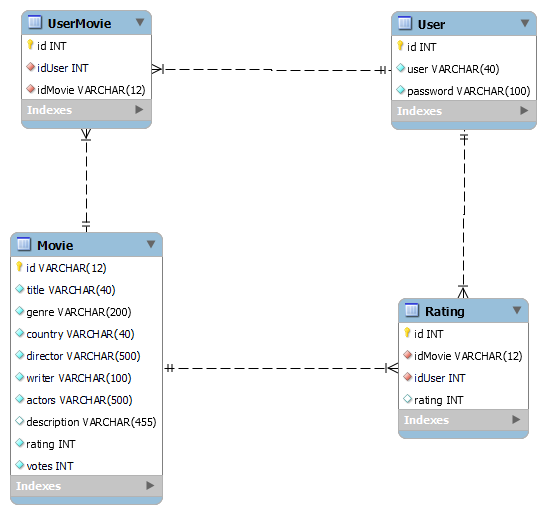
\includegraphics[width=10cm, height=10cm]{figures/diagrama db.png}}
\caption{Diagrama baza de date.}
\label{fig}
\end{figure}

\par Un lucru foarte important în dezvoltarea aplicației a fost alegerea bazei de date, am optat pentru pentru MySql versiunea 8.0. În tabelul de User voi salva datele de inregisrare a unui utilizator , în tabelul Movie sunt prezente datele care descriu un film prin coloanele: title,genre,country,directors,writers,actors,description,votes și rating, în tabelul Rating salvez datele unui rating dat de un user pe laga valoare ratingului salvez și id-urile de la film și user pentru a știi cine da rating și la ce film totodată pe partea de back-end fac și o actualizare a rating ului și numărului de voturi din tabelul Movie asta pentru o a face aplicația să se miște mai rapid, iar în tabelul UserMovie salvez id ul de la un user și id ul de la un film reprezentând un film pe care utilizatorul l-a vizualizat.

\section{Server Node Js}
\label{sec:ch5sec1}

\par Serverul de Node Js este folosit pentru a se face înregistrare, login, returanrea tuturor filmelor care conțîn un numit sub titlu, adăugarea unui film la lista utilizatorului, returnarea a tuturor filmelor unui utilizator și adăugarea de rating a unui film. Cu ajutorul pachetului Express se stabilesc rutele și se pornesc serverul. Când se face un request pe o ruta, se apelează funcția asignată din Service, care are rol de a modela datele in funcție de cum avem nevoie. Pentru a comunica cu baza de date ne folosim de Repository, acesta face legătură cu baza de date.

\par Standardul REST („representational state transfer”) a fost creat pentru a ghida design-ul și arhitectură serviciilor web. REST descrie cum ar trebui să se comporte internetul. Orice serviciu care reușește să se încadreze în parametrii și regulile descrise de acest standard se numește un serviciu RESTful.  Atunci când o cerere de client se face printr-un API RESTful, acesta transferă o reprezentare a stării resursei către solicitant sau punct final. Aceste informații sau reprezentări sunt livrate într-unul din mai multe formate prin HTTP: JSON (Javascript Object Notation), HTML, XLT, Python, PHP sau text simplu. JSON este cel mai popular limbaj de programare folosit, deoarece, în ciuda numelui său, este limbaj-agnostic, precum și lizibil atât de oameni, cât și de mașini.Altceva de reținut: anteturile și parametrii sunt, de asemenea, importanți în metodele HTTP ale unei cereri HTTP RESTful API, deoarece conțîn informații importante de identificare referitoare la metadatele cererii, autorizarea, identificatorul uniform al resurselor (URI), cache, cookie-uri. Există anteturi de solicitare și anteturi de răspuns, fiecare cu propriile informații de conexiune HTTP și coduri de stare.

\par Serverul respectă standardul REST API. Crearea entităților se face cu PUT, interogările cu GET, ștergerea cu DELETE, iar restul operațiilor cu POST. Specificațiile API în format OpenAPI se pot găsi la documentație API

		\begin{figure}[htbp]
			\centerline{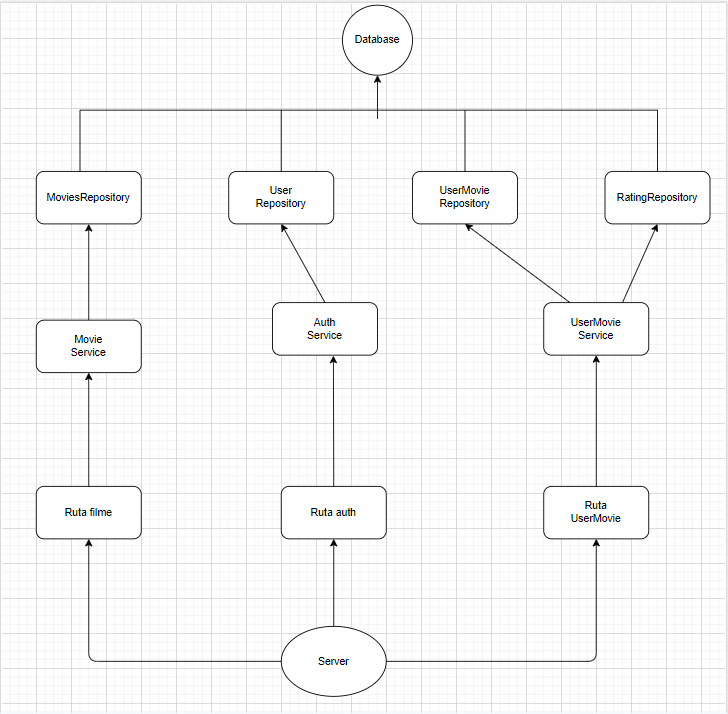
\includegraphics[width=13cm, height=10cm]{figures/diagrama clase node js.png}}
			\caption{Arhitectura server Node Js .}
			\label{fig}
		\end{figure}

\subsection{Inregistrare}
\par Procesul de înregistrare este unul simplu, pașii fiind următorii:
\begin{enumerate}
  	\item Se trimit datele către server
	\item Se validează datele primite	
	\item Dacă datele sunt valide se verifică dacă numele utilizatorului se află în baza de date deoarece numele trebuie să fie unic pentru fiecare utiliztor
	\item Dacă totul este bine până la acest pas se face has la parolă pentru o mai bună securitate
		\begin{figure}[htbp]
			\centerline{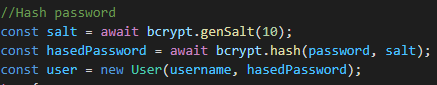
\includegraphics[width=15cm, height=4cm]{figures/hasparola.png}}
			\caption{Has la parola.}
			\label{fig}
		\end{figure}
	\item Următorul pas este de a apela functția din repositoy care adaugă un user in baza de date.
		\begin{figure}[htbp]
			\centerline{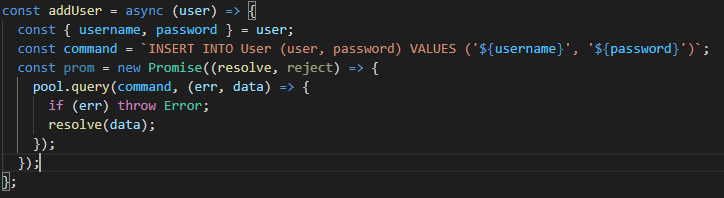
\includegraphics[width=19cm, height=6cm]{figures/adaugare user.png}}
			\caption{Adaugare user in baza de date.}
			\label{fig}
		\end{figure}	
	\item Dacă adăugarea s-a efectuat cu succes se returneaza un messaj de succes altfel se returnează un mesajul de eroare.
\end{enumerate}

\subsection{Autentificare}

\par Pașii pentru procesul de autentificare sunt următorii

	\begin{enumerate}
	
	\item Se trimit datele catre server
	
	\item Se valideaza datele primite
	
	\item Se verifica daca username-ul se afla in baza de date
			
		\begin{figure}[htbp]
		
		\centerline{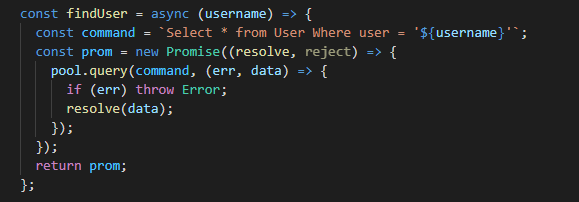
\includegraphics[width=19cm, height=6cm]{figures/cautare user.png}}
		
		\caption{Cautare dupa username in baza de date}
		
		\label{fig}
		
		\end{figure}

\item Daca se găsește user-ul in baza de date se verifică parola trimisă in requst cu cea din baza de date apoi se trimite raspunsul in functie de potrivirea celor doua parole, daca rapunsul este valid se va trimite id-ul user-ului care va reprezenta token-ul pentru front-end, daca parolele nu corespund se va trimite status 400 si un mesaj de eroare.

	\begin{figure}[htbp]

		\centerline{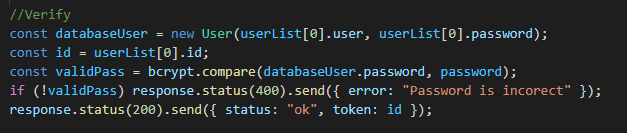
\includegraphics[width=19cm, height=6cm]{figures/verificare login.png}}
	
		\caption{Verificare parola si trimitere raspuns}
	
		\label{fig}

	\end{figure}

\end{enumerate}


\subsection{Lista filmelor care contin un subtitlu}
\par Pașii pentru returnarea listii sunt:
\begin{enumerate}
  	\item După ce se apelează ruta specifică se ia din body titlul
  	\item Se apelează functioa din repository care returnează lista
  	\item În repository se iau toate filmele din baza de date apoi se parcurg pentru a păstra doar filmele care conțin subtitlul dat.
		\begin{figure}[htbp]
			\centerline{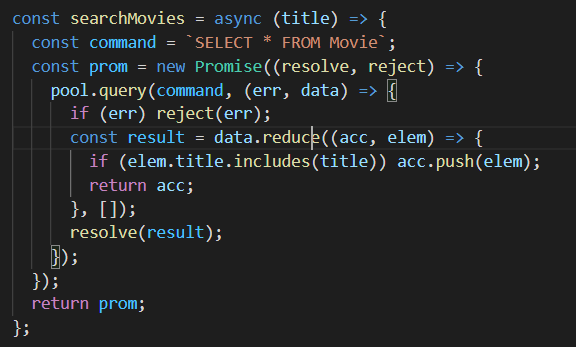
\includegraphics[width=19cm, height=6cm]{figures/cautarea filme.png}}
			\caption{Functia din repository care cauta filmele}
			\label{fig}
		\end{figure}	
\end{enumerate}

\subsection{Adaugarea unui film la lista}
\par Pașii pentru adăugare sunt:
\begin{enumerate}
  	\item Exista o ruta care trebuie sa primeasca intr-un body id-ul user-ului si id-ul unui film
  	\item Se apelează funcția din service respectivă rutei
	\item Se adaugă cele două id uri în baza de date
  	\item În cazul unei erori se returnează codul 400, iar dacă totul s-a executat așa cum trebuie se returnează codul 200 și statusul true.
		\begin{figure}[htbp]
			\centerline{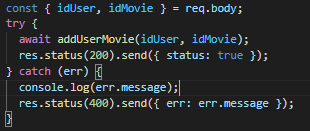
\includegraphics[width=10cm, height=6cm]{figures/adaugare film lista.png}}
			\caption{Functia pentru ruta de adaugat filme}
			\label{fig}
		\end{figure}	
	\item  În cazul în care se dorește ștergerea filmului respectiv din lista se apelează ruta "/del" cu cele 2 id-uri
\end{enumerate}


\subsection{Acordare rating}
\par Pașii pentru adaugare sunt:
\begin{enumerate}
  	\item Există o ruta care trebuie să primească într-un body id-ul user-ului , notă dată și id-ul filmului
  	\item Se apelează funcția din service respectivă rutei
	\item Se adauga cele doua id uri si nota in baza de date 
	\item În baza de date cu filme se modifică la id-ul filmului: se incrementeaza cu unu numărul de votanți și se adună la rating notă dată, acest lucru ajută la calcularea mediei generale a filmului fără a mai face un select cu toate notele unui film.
  	\item În cazul unei erori se returnează codul 400, iar dacă totul s-a executat așa cum trebuie se returnează codul 200 și statusul true.
		\begin{figure}[htbp]
			\centerline{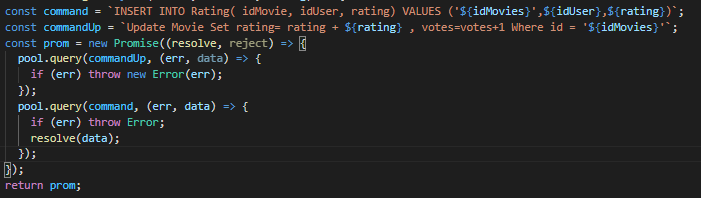
\includegraphics[width=15cm, height=5cm]{figures/functie rating.png}}
			\caption{Functia pentru ruta de adaugat filme}
			\label{fig}
		\end{figure}	
	\item  În cazul în care se dorește ștergerea filmului respectiv din lista se apelează ruta "/del" cu cele 2 id-uri
\end{enumerate}

\section{Server Flask}
\label{sec:ch5sec1}

\par Seveverul scris cu ajutorul framework-ului Flask este cel care face recomandări pentru un film sau pentru o lista de filme. La pornirea acestui server trebuie să se aștepte un anumit timp deoarece la pornire acesta ia toate datele de la baza de date apoi le procesează și calculează matricea de scoruri, face toate acestea pentru că atunci când un client cere recomandări pentru un film răspunsul să fie minim și să nu fie nevoie să facă toate aceste calcule. Există un dezanjantaj la această metodă, dacă intervin modificări la baza de date în acest timp nu vor influență scorurile, de exemplu dacă un film va fi votat cu multe voturi nu se regăși în scorul final sau dacă un film este șters din baza de date algoritmul din acest server încă îl poate recomandă. Există totuși variante pentru aceste probleme, se poate creea o funcție care să reîncarce datele iar la apelarea aceesteia să se recalculeze matricele de scoruri, iar o a două varianta puțîn mai neconvetionala se poate opri și reporni server ul acesta recalculand scorurile. Primul lucru pe care îl face serverul după citire este procesarea datelor, după care creează sacul de cuvinte și vectorii care reprezintă filmele, următorul pas fiind calcularea scorului.Server-ul are două rute una în care returnează recomandaripentru un film și o ruta care returneza recomandări pentru o lista de filme.
\par Pentru a face recomandări pentru un film algoritumul ia din linia din matricea de scoruri cele mai mari n scoruri, n reprezentând numărul de filme pe care algoritmul trebuie să îl recomande, apoi returnează o lista cu detaliile filmelor. Atunci când se cere recomandări pentru o lista de filme algoritmul ia din matricea de scoruri mai multe filme pentru fiecare film, la final sortandu-le după scor și returnează n filme cu cele mai bune scoruri.
\begin{figure}[!h]
			\centerline{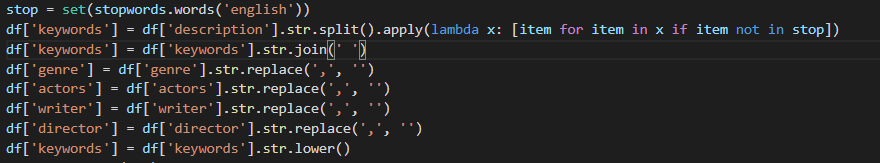
\includegraphics[width=15cm, height=6cm]{figures/prelucrare.png}}
			\caption{Prelucrarea datelor}
			\label{fig}
		\end{figure}

\begin{figure}[!h]
			\centerline{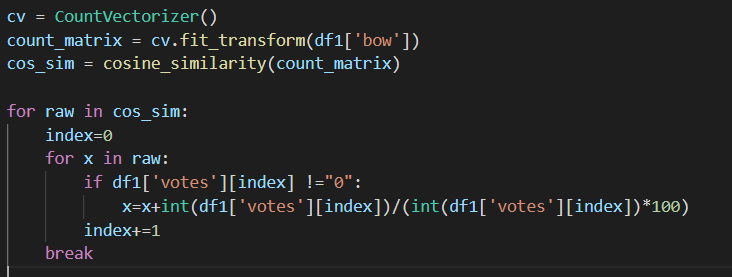
\includegraphics[width=15cm, height=6cm]{figures/calculare scoruri.png}}
			\caption{Calcularea matricii de scoruri}
			\label{fig}
		\end{figure}

\section{Front-end}
\label{sec:ch5sec1}

\par Front-endul este reprezentat de un site web scris cu ajutorul framework-ului React Js. Proiectul este împărțit pe pagini care la rândul lor conțîn diferite componente. Această metodă a componentelor este foarte utilă atunci când se refolosește cod, este că și o funcție care este scrisă o singură dată dar este apelată în mai multe locuri. Există două tipuri de pagini, publice și private, cele publice pot fi accesate de un user fără a fi neoie de autentificare, iar cele publice necesită o autentificare. Stilizarea site-ului web se face cu ajutorul CSS-ului în două moduri, una fiin prin importarea fișierelor de CSS în componente și pagini și una cu ajutorul injectării în componente cu ajutorul JavaScript. Pentru a putea naviga între pagini există un router în care se specifică pentru fiecare ruta din aplicație pagină care trebuie să fie afișată și dacă această este publică sau privată, în cazul in care este privată iar user-ul nu s-a autentificat acesta va fi redirecționat la una din rutele publice. Acesta respectă standardul REST și se folosește de librăria axios pentru a face cereri către server.
\subsection{Autentificare si inregistrare}
\par Pașii sunt:

\begin{enumerate}
  	\item Atunci când utilizatorul accesează site-ul web este redirecționat la pagină de autentificare unde trebuie să introducă userul și parolă
	\item Dacă nu are un cont poate apasă re butonul de înregistrare unde va fi redirecționat către pagină de înregistrare:
		\begin{enumerate}
		  	\item După completarea folmularului de înregistrare și pasărea butonului datele vor fi validate
			\item Următorul pas este de a trimite datele la server
			\item Dacă se primește status 200 userv-ul va fi redirecționat către pagină de autentificare
			\item Dacă se primește alt status se va afișa eroarea, iar pașii de înregistrare trebuie repetați până se introduc date valide 
		\end{enumerate}
	\item După ce toate datele de autentificare au fost introduse ele se trimit la server, iar dacă datele sunt corecte se primește că și răspuns token-ul care fă fi salvat în memorie și utilizatorul va fi redirecționat către pagină principala
	\item Dacă de la server se primește răspuns negativ se va afișa eroarea, iar pașii trebuie repetați.
\end{enumerate}

\subsection{Cautare filme}
\par Pașii sunt:

\begin{enumerate}
  	\item După ce utilizatorul s-a autentificat acesta este redirecționat către pagină principala unde poate caută filme după titlu
	\item După ce introduce titlul pe care acesta îl câtă și apasă pe buton vor apărea toate filmele care în titlu conțin șirul introdus de utilizator
	\item Fiecare film are două opțiuni, mai multe detalii și adaugă la lista
	\item Dacă se alege opțiunea de mai multe detalii acesta va fi redirecționat către pagină unde poate vedea detaliile explicite ale filmului și poate cel mai important se face și o recomandare de patru filme pentru filmul respectiv.Tot pe această pagină se poate da un rating filmului astfel influențând rating-ul filmului.
	\item Dacă se alege opțiunea de adăugare la lista acesta se va adaugă la lista utilizatorului, vizibilă pe altă pagină a aplicației, iar această opțiune va dispărea
\end{enumerate}


\subsection{Lista cu filme}

\begin{enumerate}
  	\item Pe această pagină se încarcă toate filmele utilizatorului cu două opțiuni, se poate șterge filmul din lista sau se poate face redirecționare către pagină cu detalii explicite ale filmului.
	\item Tot pe această pagină se poate creea o lista pentru care se poate face recomandări de filme:
			\begin{enumerate}
		  	\item Se pasă pe butonul cu plus, iar titlul filmului va apărea într-o lista poziționată în partea de sus a pagini, filmul poate fi și deselectat deoarece după adăugare va apărea un buton pentru această opțiune
			\item  După ce toate filmele au fost selectate se apasă pe buton
			\item Se vor afișa toate filmele recomandate pentru lista de filme aleasă
		\end{enumerate}
	


\end{enumerate}